\documentclass[12pt]{article}

% --- Paquetes comunes ---
\usepackage[utf8]{inputenc}
\usepackage[T1]{fontenc}
\usepackage[spanish]{babel}
\usepackage{amsmath}
\usepackage{amssymb}
\usepackage{hyperref}
\usepackage{graphicx} % <--- ¡NUEVO! Paquete para incluir imágenes

% --- Configuración de márgenes (opcional, para una mejor presentación) ---
\usepackage[margin=2.5cm]{geometry}

% --- Información del documento ---
\title{Práctica 1: Nombre de tu Tarea}
\author{
  Nombre del Estudiante \\
  \texttt{corredsdholaaaao@ejemplo.com}
  \and
  Nombre del Docente \\
  Materia
}
\date{\today}

\begin{document}

% --- Portada ---
\maketitle
\thispagestyle{empty} % No pone el número de página en la portada

\clearpage
\pagenumbering{arabic} % Empieza a numerar las páginas a partir de aquí

\section{Introducción}
\label{sec:introduccion}
Este documento presenta la resolución de la Práctica 1. En esta sección se describen los objetivos de la práctica y se contextualiza el problema a resolver. El propósito principal es aplicar los conceptos aprendidos en clase para demostrar el entendimiento de los temas.

\section{Desarrollo de la Práctica}
\label{sec:desarrollo}
Aquí se detalla el trabajo realizado para la práctica. Puedes usar subsecciones para organizar tu contenido de manera lógica.

\subsection{Problema 1}
\label{subsec:problema1}
Describe el primer problema y el enfoque que usaste para resolverlo. Puedes incluir código, si es necesario, usando el entorno \texttt{verbatim} o el paquete \texttt{listings}.

\begin{verbatim}
# Código de ejemplo en Python
def saludo(nombre):
    print(f"Hola, {nombre}")

saludo("mundo")
\end{verbatim}

\subsection{Problema 2}
\label{subsec:problema2}
Explica el segundo problema y la metodología que aplicaste. Usa ecuaciones para mostrar tus cálculos. Las ecuaciones pueden ser inline, como $E=mc^2$, o en un entorno separado para que se vean mejor:

\begin{equation}
    x = \frac{-b \pm \sqrt{b^2 - 4ac}}{2a}
    \label{eq:formula_cuadratica}
\end{equation}
La ecuación \eqref{eq:formula_cuadratica} es un ejemplo de cómo se pueden insertar fórmulas matemáticas.

\section{Inclusión de Imagen}
Para ilustrar un punto importante de la práctica, hemos incluido una imagen. Se puede hacer referencia a la misma en el texto, como se ve en la Figura \ref{fig:mi_imagen}.

\begin{figure}[h!]
    \centering
    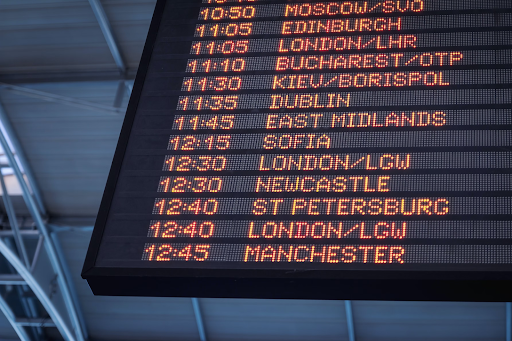
\includegraphics[width=0.7\linewidth]{Imagen.png} % <--- ¡NUEVO! Comando para insertar la imagen
    \caption{Una imagen para ilustrar el trabajo de la práctica.}
    \label{fig:mi_imagen}
\end{figure}

\section{Conclusiones}
\label{sec:conclusiones}
En esta sección se resumen los resultados obtenidos en la práctica. Discute si los objetivos iniciales se cumplieron y cualquier aprendizaje o dificultad que encontraste durante el proceso.

\end{document}